\section{Spannungsregelung}
Unter Spannungsstabilität versteht man die Fähigkeit eines Stromversorgungssystems, an allen Bussen im System konstante Spannungen aufrechtzuerhalten, nachdem es einer Störung aus einem gegebenen Betriebszustand ausgesetzt wurde.


\subsection{Spannungskollaps}

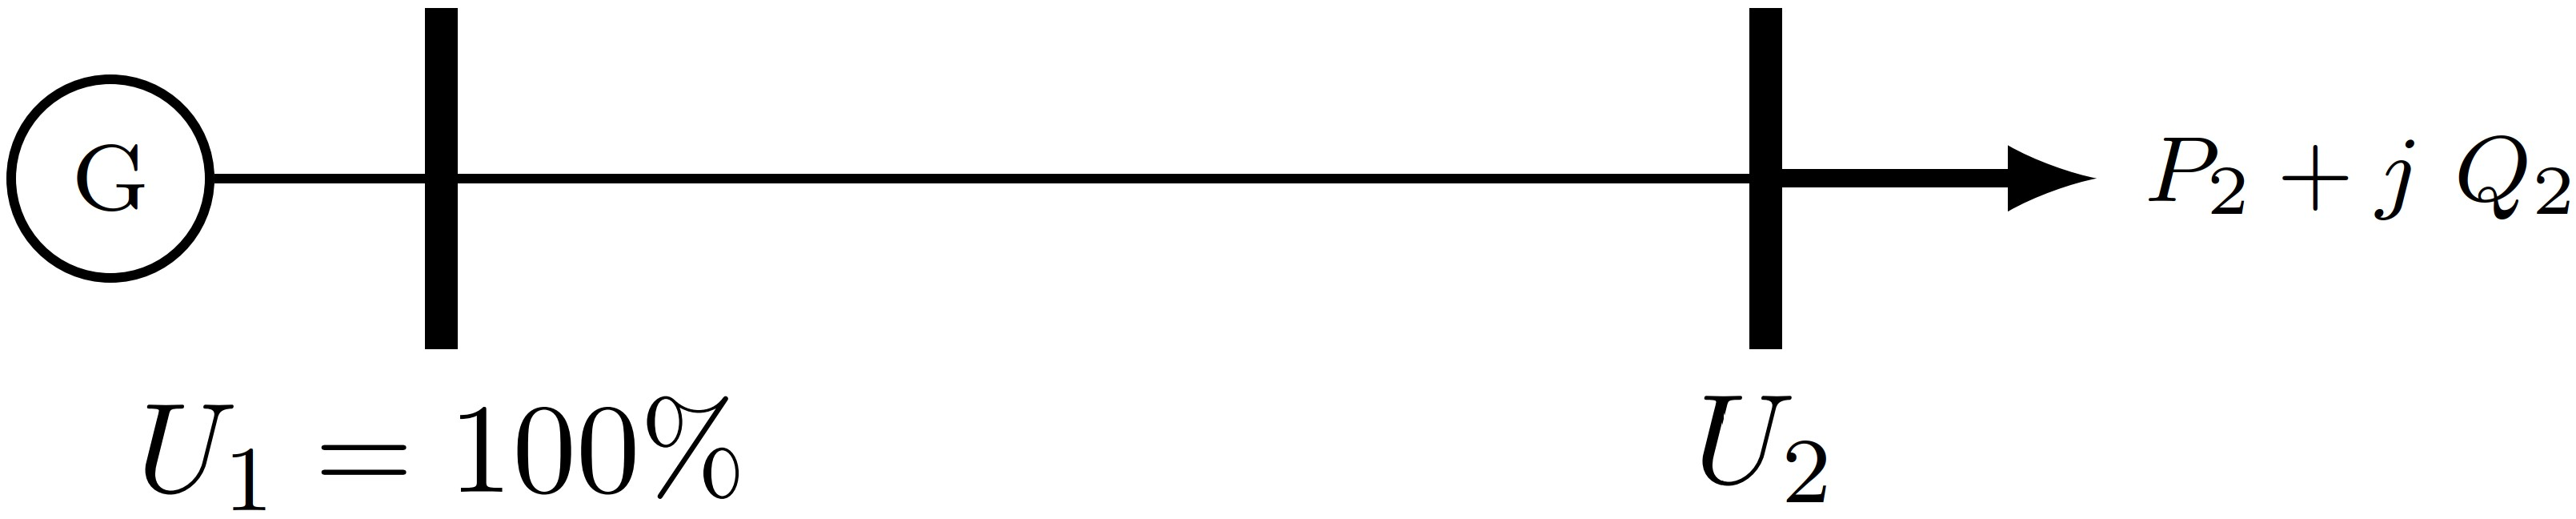
\includegraphics[width=0.68\columnwidth, align=c]{images/Spannungsregelung_2.jpg}

\vspace{0.15cm}


\subsection{}


\subsection{}


\subsection{}


\subsection{}


\subsection{}


\subsection{}


\subsection{}


\subsection{}


\subsection{}


\subsection{}
